\documentclass[a4paper]{article}

%% Page Size and Margins
\usepackage[a4paper,top=3cm,bottom=2cm,left=2cm,right=2cm,marginparwidth=1.75cm]{geometry}

%% Useful packages
\usepackage{graphicx}
\usepackage{fancyhdr}
\usepackage{hyperref}

%%\usepackage{amsmath}
%%\usepackage[colorinlistoftodos]{todonotes}
%%\usepackage[colorlinks=true, allcolors=blue]{hyperref}
%%\usepackage{caption}
%%\usepackage{subcaption}
%%\usepackage{sectsty}
%%\usepackage{apacite}
%%\usepackage{float}
%%\usepackage{titling} 
%%\usepackage{blindtext}
%%\usepackage[square,sort,comma,numbers]{natbib}
%%\usepackage[colorinlistoftodos]{todonotes}
%%\usepackage{xcolor}
%%\definecolor{darkgreen}{rgb}{0.0, 0.4, 0.0}

%% Document Begin
\begin{document}

%% titlepage
\begin{titlepage}
\vspace*{100px}
\newcommand{\HRule}{\rule{\linewidth}{0.5mm}} 	
\center 
 
% Fisrt row
{ \huge \bfseries Icom-Proxy}
\vspace*{50px}

% Program info
\HRule \\[0.8cm]

\textsc{\normalsize \emph {To run multiple programs on just one Icom-radio}}\\[0.8cm]

\HRule \\[1cm]

%%Picture
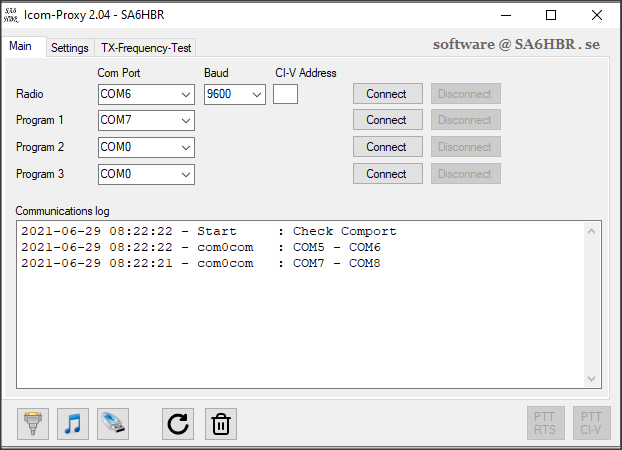
\includegraphics[width=0.6\textwidth]{../image/Icom_Proxy.png}\\[3cm] 

{\large \today}\\[2cm]
\textsc{ \huge \bfseries SA6HBR}\\[1cm]

\vfill 
\end{titlepage}

\pagestyle{fancy}
\fancyhf{}
\lhead{\today}
\rhead{SA6HBR}

%%\lhead{Guides and tutorials}
\cfoot{ \thepage}

%% Section English
%%\section*{English}

%%Simple program for displaying serial communication
%%\newpage

%% Section Svenska
\section*{Svenska}

Detta program kan man använda om man vill köra flera program med en Icom-Radio.
\newline
\newline
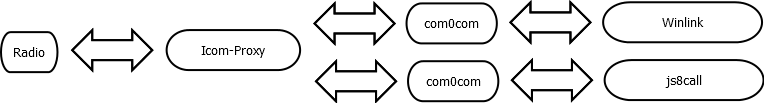
\includegraphics[width=0.8\textwidth]{../image/Diagram1.png}\\[0.2cm] 
Normal inkoppling är att "Icom-Proxy" kopplas till radion och via komportspar till programmen som skall samtidigt köras.
Komportspar kan skapas med hjälp av com0com.
\newline
\newline
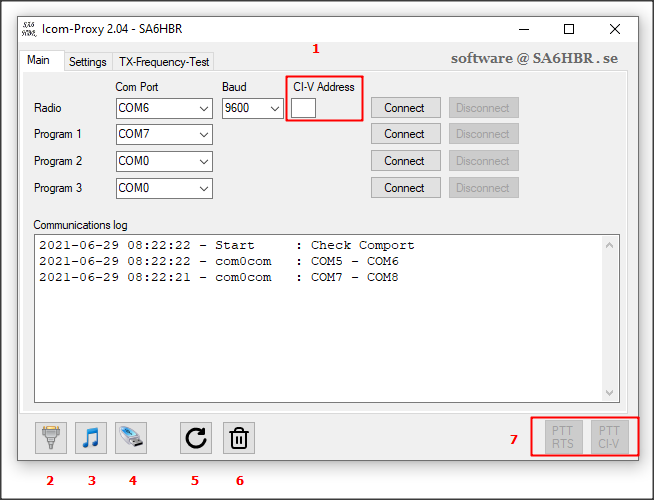
\includegraphics[width=1\textwidth]{../image/Icom_Proxy_main.png}\\[0.1cm] 


\begin{enumerate}   
\item Radions adress hittas normalt direkt när man trycker på Connect, men om inte så får man fylla i det. Exempel IC-728 har adressen 38.
\item Genväg till com0com
\item Genväg till ljudinställningarna
\item Genväg till datorns systeminställningar
\item Uppdaterar komportarna
\item Tömmer loggrutan
\item Lyser rött när PTT aktiveras
\end{enumerate}  

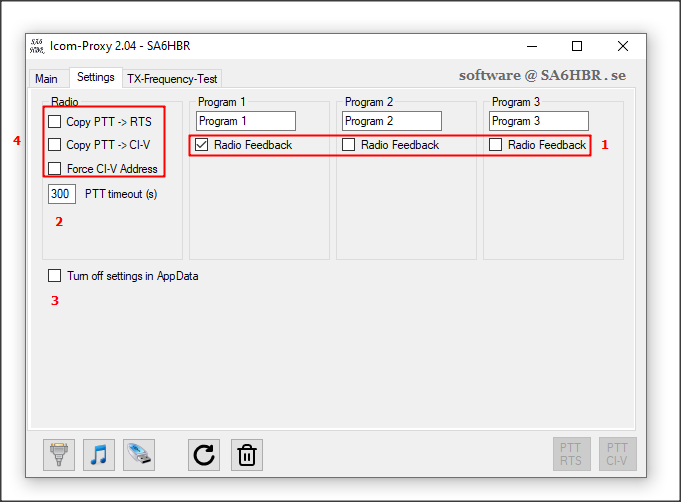
\includegraphics[width=1\textwidth]{../image/Icom_Proxy_settings.png}\\[0.5cm] 


\begin{enumerate}   
\item Winlink läser inte från komporten och buffert fylls. Bocka endast i rutan om ni använder program som kräver dubbelriktad kommunikation, exempelvis js8call.
\item Väljer den tid som längst PTT skall vara aktiv.
\item Inställningarna sparas inte om man bockar ur, som kan vara bra om man vill testa lite nya inställningar. 
\item I fall programmen inte har rätt inställningar för din Icom, så kan man testa dessa inställningar.
\end{enumerate}  

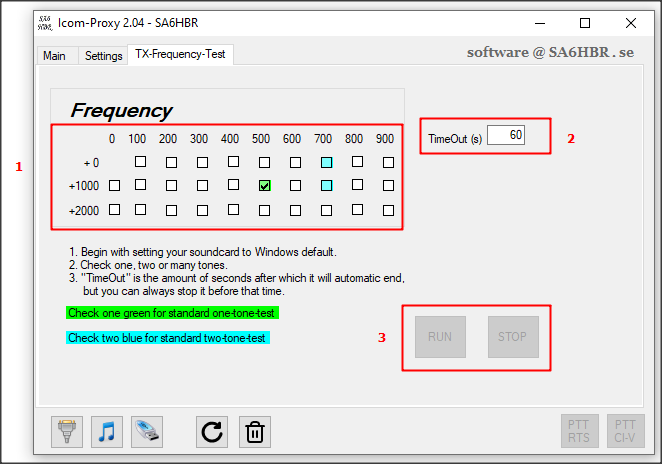
\includegraphics[width=1\textwidth]{../image/Icom_Proxy_frequence_test.png}\\[0.5cm] 


\begin{enumerate}   
\item Välj en eller flera frekvenser som man vill testa uteffekten med. Flera toner samtidigt ger lägre uteffekt.
\item Välj den tid som tonen skall vara. Går att avbryta innan. Längre tid kan göra att det tar längre tid innan PTT aktiveras.
\item Start och Stopp
\end{enumerate}  

Tonen spelas med datorns standardljudkort.

\vspace*{50px}
\newpage


%% Section  Useful Links
\section*{Useful Links}

* Null-modem emulator (com0com) \href{https://sourceforge.net/projects/com0com/}{https://sourceforge.net/projects/com0com/}. 

%% Section License
\section*{License}

GNU General Public License v3.0


\end{document}